% =====================================================================
%  Blog #1 — „Most n-gram → transformer" (pełna wersja LaTeX).
%  Baza: draft.tex (skondensowany) + proza blogdraft/most-ngram-transformer.md + konspekt.
%  Formatka: slay-paper (formatka/slayer.sty).  Status: DRAFT — masterujemy.
% =====================================================================
\documentclass[11pt,a4paper]{article}
\usepackage{formatka/slayer}

\title{Dlaczego 6-gram prawie dorównuje transformerowi\\
\large --- i czemu to \emph{nie} znaczy, że wygrywa}
\author{kolektyw \textbf{Slayer} \\ \texttt{github.com/slayerlabs/micro-models}}
\date{czerwiec 2026}

\begin{document}
\maketitle

\begin{abstract}
\noindent\textbf{TL;DR.} Na char-level korpusie muzyki \textbf{n-gram rzędu 6 osiąga perplexity 3,90 --- niemal jak nasz mini-transformer (3,80)}. Brzmi jak „to po co komu transformery?". Odpowiedź: perplexity to tylko \emph{jeden z trzech zasobów}. Gdy dołożymy \textbf{pamięć} i \textbf{obliczenia}, n-gram i transformer okazują się \textbf{przeciwnymi rogami} tego samego trójkąta --- a różnicą, której perplexity nie widzi, jest \textbf{generalizacja}. \emph{Status: DRAFT; kod i wagi otwarte.}
\end{abstract}

\section{Jeden cel, spektrum mechanizmów}
Wytrenowaliśmy malutki transformer na melodiach --- cztery warstwy, $\sim$0,8 mln parametrów, trening w minuty na CPU. Potem, dla porównania, zwykły \textbf{n-gram}: technologię z lat 90., która tylko \emph{zlicza}. I n-gram \textbf{prawie go dogonił}. Więc po co komu transformery, GPU, miliardy parametrów? Odpowiedź okazała się ciekawsza, niż się spodziewaliśmy --- i o niej jest ten tekst.

Zacznijmy od tego, co łączy zawodników. Każdy model języka robi to samo: przewiduje następny token, $p(\text{następny}\mid\text{poprzednie})$. n-gram i transformer to nie „stary" i „nowy" model --- to dwa \textbf{mechanizmy} tego samego celu: \textbf{twarde zliczanie} vs \textbf{miękka uwaga}. Między nimi leży ciągłe spektrum.

To są \textbf{mikro-modele}: sieci dość małe, by zrozumieć je od początku do końca. Zeszliśmy na najmniejszy, w pełni audytowalny koniec --- \textbf{poziom znaku}, korpus melodii (jigi w notacji ABC) --- wszystko na \emph{jednym} podziale train/val, więc perplexity (= jak bardzo model \emph{zdziwił się} prawdziwym następnym znakiem; niżej = lepiej) jest bezpośrednio porównywalne. Cel mają ten sam --- czas poznać trzech zawodników.

\section{Trzej zawodnicy}
\begin{itemize}
  \item \textbf{n-gram} --- \emph{gigantyczny notes ze zliczeniami}: „po \texttt{abc} w 70\% przypadków padło \texttt{d}". Czyta $p$ z tablicy po oknie $k$ znaków. Szybki, ale notes puchnie wykładniczo i nie radzi sobie z frazą, której nie zapisał. Używamy \textbf{interpolacji rzędów} (1\,--\,6-gram z gładkim backoffem; nowsze warianty skalują to do bilionów tokenów \cite{infinigram}).
  \item \textbf{NPLM} \cite{nplm} --- ktoś, kto zamiast notesu \emph{nauczył się wzorców} z ostatnich $N$ znaków (mały MLP nad embeddingami). Stałe okno jak n-gram, ale \textbf{uczy się reprezentacji, nie tablicy} --- działa też na nowych kombinacjach.
  \item \textbf{mini-GPT} \cite{vaswani} --- model, który \emph{sam decyduje, na które wcześniejsze znaki patrzeć} i jak daleko (to właśnie uwaga). Zmienne, długie okno zamiast sztywnego.
\end{itemize}
Cel mają identyczny --- różni ich tylko \emph{jak} sięgają po przeszłość. Zmierzmy ich: kto zgaduje lepiej?

\paragraph{Jak interpolujemy n-gram.} Ważona średnia oszacowań z każdego rzędu, renormalizowana po rzędach, których kontekst \emph{był} w treningu:
\[
P(\text{znak}\mid\text{ctx}) = \frac{\sum_o w_o\,p_o(\text{znak}\mid\text{ostatnie } o \text{ znaków})}{\sum_o w_o},\qquad w_o = 2^{o}.
\]
Najdłuższy widziany kontekst dominuje; gdy go brak --- backoff na krótszy. Rząd 0 (unigram, add-$k$) zawsze aktywny, więc żaden znak nie dostaje zera. Prosty, jawny schemat (nie Kneser--Ney); wagi nieuczone.

\section{Wynik 1: perplexity --- i niespodzianka}
\begin{figure}[h]
  \centering
  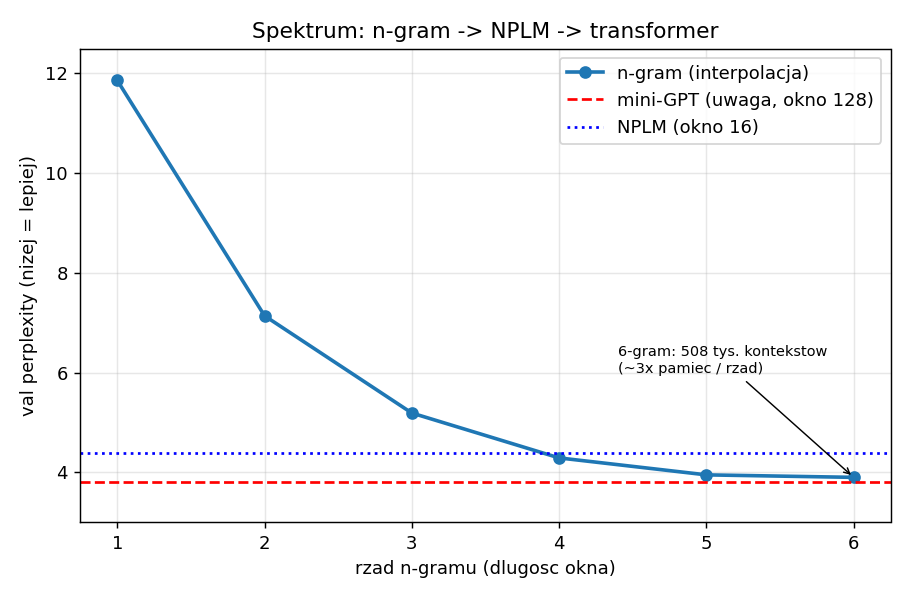
\includegraphics[width=0.82\linewidth]{chart3_spectrum.png}
  \caption{Spektrum: n-gram (rośnie z rzędem) dobija do mini-GPT; NPLM pomiędzy.}
  \label{fig:spektrum}
\end{figure}

\begin{table}[h]
  \centering
  \caption{Perplexity walidacyjne (jeden podział, char-level).}
  \begin{tabular}{llr}
    \toprule
    Model & mechanizm & val ppl \\
    \midrule
    n-gram rząd 1 & zliczanie, okno 1 & 11,86 \\
    n-gram rząd 3 & zliczanie, okno 3 & 5,19 \\
    n-gram rząd 6 & zliczanie, okno 6 & \textbf{3,90} \\
    NPLM, okno 8 & MLP, stałe okno & 4,41 \\
    NPLM, okno 16 & MLP, stałe okno & 4,38 \\
    \textbf{mini-GPT} & uwaga, okno 128 & \textbf{3,80} \\
    \bottomrule
  \end{tabular}
\end{table}

n-gram poprawia się z rzędem (11,86 $\to$ 3,90) i \textbf{dobija do GPT} przy rzędzie 5\,--\,6. Na samym perplexity to prawie remis. Więc transformer zbędny? Nie --- bo perplexity to \emph{jedna} liczba. Pytanie brzmi: \textbf{co ona przemilcza?}

\section{Wynik 2: trzy zasoby, nie jedna liczba}
\subsection{Pamięć}
\begin{table}[h]
  \centering
  \begin{tabular}{ll}
    \toprule
    Model & co przechowuje \\
    \midrule
    n-gram rząd 6 & \textbf{508 tys. kontekstów} (rośnie $\sim$2\,--\,3$\times$ na rząd) \\
    NPLM, okno 8 & $\sim$41 tys. parametrów \\
    mini-GPT & $\sim$800 tys. parametrów \\
    \bottomrule
  \end{tabular}
\end{table}
n-gram kupuje jakość \textbf{pamięcią rosnącą lawinowo}: z 52 kontekstów (rząd 1) do 508 tys. (rząd 6), przy malejącym zysku (rz.\ 5$\to$6: ppl $3{,}95\to3{,}90$).

\subsection{Obliczenia --- ile FLOPs na jeden token}
Transformer (4 warstwy, $d=128$, kontekst $T=128$), dominujące mnożenia macierzowe na warstwę:
\begin{table}[h]
  \centering
  \begin{tabular}{lrr}
    \toprule
    Składnik & wzór & MAC \\
    \midrule
    QKV proj & $3d^2$ & 49\,152 \\
    atencja  & $2dT$  & 32\,768 \\
    out proj & $d^2$  & 16\,384 \\
    MLP      & $8d^2$ & 131\,072 \\
    \midrule
    \textbf{na warstwę} & & $\approx$229K \\
    \textbf{$\times 4$ + głowica} & & $\approx$0,92M MAC $\approx$ \textbf{\textasciitilde1,8M FLOPs/token} \\
    \bottomrule
  \end{tabular}
\end{table}

\begin{table}[h]
  \centering
  \begin{tabular}{ll}
    \toprule
    Model & obliczenia / token \\
    \midrule
    n-gram $\le 6$ & $\sim$7 odczytów z tablicy + $\sim$20 operacji (arytmetyka $\approx 0$) \\
    NPLM, okno 8 & $\sim$79 tys. FLOPs \\
    mini-GPT & \textbf{$\sim$1,8 mln FLOPs} (rośnie z długością kontekstu) \\
    \bottomrule
  \end{tabular}
\end{table}

Transformer robi \textbf{$\sim$23$\times$ więcej} arytmetyki niż NPLM i \textbf{$\sim$90\,000$\times$ więcej} niż n-gram. \textbf{Compute jest niemal odwrotnością pamięci.} \emph{(To szacunki dominujących mnożeń macierzowych --- pomijamy softmax, normalizacje i bias; rząd wielkości się trzyma.)}

\paragraph{Puenta (i tytuł serii).} Te operacje to \textbf{mnożenie i dodawanie --- arytmetyka z liceum}. GPT nie robi egzotycznej matematyki; robi \emph{miliony prostych operacji na jeden znak}. Trudność nie leży w magicznej matmie --- leży w \textbf{SKALI}. „High school is all you need" do zrozumienia \emph{mechanizmu}; reszta to inżynieria skali.

\subsection{Generalizacja}
n-gram \textbf{nie ekstrapoluje}: nieznany kontekst $\to$ backoff do krótszego, w skrajności do unigramu --- \emph{rekombinuje widziane, nie tworzy nic dla nowego wzorca}. Sieci neuronowe uogólniają po podobieństwie w przestrzeni embeddingów \cite{knnlm}. Krótko: \textbf{n-gram pamięta, nie uogólnia}. Te trzy osie --- jakość, pamięć, obliczenia --- składają się w jeden obraz.

\section{Trójkąt: jakość \texorpdfstring{$\leftrightarrow$}{<->} pamięć \texorpdfstring{$\leftrightarrow$}{<->} obliczenia}
\textbf{„Lepszy model" to nie jedna liczba --- to trójkąt: jakość $\leftrightarrow$ pamięć $\leftrightarrow$ obliczenia}, a w tle \textbf{generalizacja}:
\begin{figure}[h]
  \centering
  \begin{tikzpicture}
    \begin{axis}[
        width=0.8\linewidth, height=6cm, xmode=log, ymode=log,
        xlabel={obliczenia (FLOPs/token, log)}, ylabel={pamięć (pozycje/parametry, log)},
        grid=both, grid style={gray!20},
        nodes near coords, point meta=explicit symbolic,
        every node near coord/.append style={anchor=west, font=\small},
        enlarge x limits=0.3, enlarge y limits=0.25]
      \addplot[only marks, mark=*, mark size=3pt] coordinates {
        (7,508000)       [n-gram]
        (79000,41000)    [NPLM]
        (1800000,800000) [mini-GPT]};
    \end{axis}
  \end{tikzpicture}
  \caption{Przeciwne rogi: \textbf{n-gram} tani w obliczeniach, drogi w pamięci; \textbf{transformer} drogi w obliczeniach, zwarty; \textbf{NPLM} = most (tani i zwarty, ograniczony stałym oknem).}
  \label{fig:trojkat}
\end{figure}

\noindent n-gram i transformer to \textbf{przeciwne rogi} tego samego trójkąta; NPLM pokazuje, że między nimi jest ciągłe, sensowne spektrum.

\section{Uczciwie: czemu n-gram wygląda aż tak dobrze?}
Bo muzyka jest \textbf{repetytywna} --- wiele 6-gramów z val występuje \emph{dosłownie} w train, więc n-gram „wygrywa pamiętaniem". \textbf{Czego jeszcze NIE zmierzyliśmy:} czystego testu ekstrapolacji --- val z \emph{całkiem nowych melodii} (nie pocięty ten sam strumień). Przewidujemy, że tam n-gram siądzie (backoff do unigramu), a sieci utrzymają --- to nasz następny eksperyment. Nie udajemy, że to już pokazaliśmy.

\section{Most do praktyki Slayera (koncepcyjny)}
\textbf{Ostrzeżenie:} nie zestawiamy tych liczb z produkcyjnymi --- char-ppl na muzyce a accuracy na polskich zadaniach to \emph{różne osie}. Most jest koncepcyjny: przenosi się \textbf{ten sam cel} (predykcja następnego tokena, od char-LM po duży model) i \textbf{ta sama dyscyplina pomiaru} (held-out, dekontaminacja, brak benchmaxxingu) --- zmienia się tylko metryka. Napięcie pamięć\,vs\,generalizacja z zabawki to to samo napięcie w roadmapie: tani, składalny, suwerenny polski model i ewaluacja, której nie da się oszukać.

\section{Wnioski}
Perplexity to jeden wymiar. „n-gram czy transformer?" rozstrzyga się w \textbf{trójkącie zasobów + generalizacji}. Najtańszy compute (n-gram) płaci pamięcią i brakiem generalizacji; najlepsza generalizacja (transformer) płaci obliczeniami. Wybór mechanizmu = wybór, który zasób jest tani w Twoim zastosowaniu.

\section{Spróbuj sam}
Cały przykład jest uruchamialny na CPU w minuty:
\begin{verbatim}
git clone https://github.com/slayerlabs/micro-models
# music-experts/ : trening eksperta + generacja + porownanie n-gram/NPLM/GPT
\end{verbatim}
\textbf{Następny szczebel:} weź „good first issue", odpal benchmark lokalnie i zgłoś wynik --- jesteś w środku, z publicznym, podpisanym wkładem. \emph{Następny odcinek serii:} kompozycja małych ekspertów (stitch, ensemble) i wspólna geometria reprezentacji.

\section{Jak pracujemy (Slayer)}
\emph{Żadnej tezy bez dowodu}; publikujemy też \textbf{wyniki negatywne}; pomiary przez \textbf{adwersarialny audyt} (przy pokrewnym eksperymencie złapaliśmy tak własny błąd metryki, zanim cokolwiek ogłosiliśmy). Dwie bramki: \emph{dialektyka} pilnuje, czy rozumiemy; \emph{ewaluacja} --- czy teza jest prawdziwa.

\begin{thebibliography}{9}
\bibitem{nplm} Y.~Bengio i in. \emph{A Neural Probabilistic Language Model}. JMLR 2003.
\bibitem{vaswani} A.~Vaswani i in. \emph{Attention Is All You Need}. NeurIPS 2017.
\bibitem{knnlm} U.~Khandelwal i in. \emph{Generalization through Memorization: Nearest Neighbor LMs}. ICLR 2020.
\bibitem{infinigram} J.~Liu i in. \emph{Infini-gram: Scaling Unbounded n-gram LMs to a Trillion Tokens}. COLM 2024.
\end{thebibliography}

\end{document}
